\documentclass{a0poster}
\usepackage{fancytikzposter} 
 
\usepackage[T1]{fontenc} 
\usepackage[cp1251]{inputenc}
\usepackage[russian]{babel}
\usepackage{graphicx}
\usepackage{graphics}
\usepackage{amssymb}
\usepackage{mathtext}
\usepackage{caption}
\usepackage{subcaption}
\usepackage{setspace}
\usepackage{amsmath}
\usepackage{amsthm}
\usepackage{lscape}
\usepackage{makecell}
\usepackage{multirow}
\usepackage{ulem}
\usepackage{indentfirst}
\usepackage{enumerate}

\usepackage[margin=\margin cm, paperwidth=84.1cm, paperheight=118.9cm]{geometry}

%%%%% --------- Change here if you want ---------- %%%%%
%% margin for the geometry package, must be changed before using the geometry package
%% default value is 4cm
% \setmargin{4}

%% the space between the blocks
%% default value is 2cm
% \setblockspacing{2}

%% the height of the title stripe in block nodes, decrease it to save space
%% default value is 3cm
% \setblocktitleheight{3}

%% the number of columns in the poster, possible values 2,3
%% default value is 2
% \setcolumnnumber{3}

%% the space between two or more groups of authors from different institutions
%% used in \maketitle
% \setinstituteshift{10}

\usetemplate{4}

%% components of the templates
%% (the maximal possible numbers are mentioned as the parameters)
% \usecolortemplate{4}
% \usebackgroundtemplate{5}
% \usetitletemplate{2}
% \useblocknodetemplate{5}
% \useplainblocktemplate{4}
% \useinnerblocktemplate{2}


%% the height of the head drawing on top 
%% applicable to templates N3, 4 and 5
% \setheaddrawingheight{14}


%% change the basic colors
%\definecolor{myblue}{HTML}{008888} 
%\setfirstcolor{myblue}% default 116699
%\setsecondcolor{gray!80!}% default CCCCCC
%\setthirdcolor{red!80!black}% default 991111

%% change the more specific colors
% \setbackgrounddarkcolor{colorone!70!black}
% \setbackgroundlightcolor{colorone!70!}
% \settitletextcolor{textcolor}
% \settitlefillcolor{white}
% \settitledrawcolor{colortwo}
% \setblocktextcolor{textcolor}
% \setblockfillcolor{white}
% \setblocktitletextcolor{colorone}
% \setblocktitlefillcolor{colortwo} %the color of the border
% \setplainblocktextcolor{textcolor}
\setplainblockfillcolor{colorone!10!}
% \setplainblocktitletextcolor{textcolor}
\setplainblocktitlefillcolor{colorone!60!}
% \setinnerblocktextcolor{textcolor}
% \setinnerblockfillcolor{white}
% \setinnerblocktitletextcolor{white}
% \setinnerblocktitlefillcolor{colorthree}

%% changing the fonts
%\usepackage{cmbright}

\renewcommand\normalsize{\fontsize{32}{39.8pt}\selectfont}

%% add your packages here
\usepackage{hyperref}

\title{Stable regimes of dynamic systems with impulsive influences}
\author{Leonid Ivanovsky\\
  \textit{postgraduate student, } \\
  \textit{P.G. Demidov Yaroslavl State University}
}

\begin{document}

%%%%% ---------- the background picture ---------- %%%%%
%% to change it modify the macro \BackgroundPicture
\ClearShipoutPicture
\AddToShipoutPicture{\BackgroundPicture}

\noindent % to have the picture right in the center
\begin{tikzpicture}
  \initializesizeandshifts
  % \setxshift{15}
  % \setyshift{2}

  %% the title block, #1 - shift, the default value is (0,0), #2 - width, #3 - scale
  %% the alias of the title block is `title', so we can refer to its boundaries later
  \ifthenelse{\equal{\template}{1}}{ 
    \titleblock{47}{1}
  }{
    \titleblock{47}{1.5}
  }

  %% a logo can be added to the title block
  %% #1 - anchor relative to the title block, #2 - shift, #3 - width, #3 - file name
  % \ifthenelse{\equal{\template}{2}}{ 
  %   \addlogo[south west]{(2,0)}{6cm}{unibz_b.png}
  % }{
  %   \addlogo[south west]{(2,0)}{6cm}{unibz_w.png}
  % }

  %%%%%%%%%% ------------------------------------------ %%%%%%%%%%
  \blocknodew{37}{Dynamic system} %
  {
  	\begin{equation}
		\dot{u_j} = d(a_1u_{j-1}-a_2u_j+u_{j+1})+\lambda[-1+\alpha f(u_j(t-1)) - \beta g(u_j)]u_j, \quad j=\overline{1,3},
	\end{equation}		
	$$ u_j=u_j(t)>0, \; a_1, a_2 \in \{0, 1, 2\}, \; \lambda >> 1, \; \beta > 0, \; \alpha > 1 + \beta, $$
	$$ f(u), g(u) \in C^2(\mathbb{R}_+), \; 0 < \beta g(u) < \alpha, \; f(0) = g(0) = 1, \; \forall u \in \mathbb{R}_+; $$
	$$ f(u), g(u), uf'(u), ug'(u), u^2f''(u), u^2g''(u) = O(1/u), \; u \to +\infty. $$
  }

%%%%%%%%%% ------------------------------------------ %%%%%%%%%%
  \blocknodew[($(currenty)+(19.5,0)$)]{76}{Phase portraits in the case $ a_1 = 1, \, a_2 = 2; \, u_0 = u_1, \, u_3 = u_4 $ } %
  { 
	
\vspace{0.1cm}	
			
	\begin{minipage}[h]{0.37\linewidth}
	\center{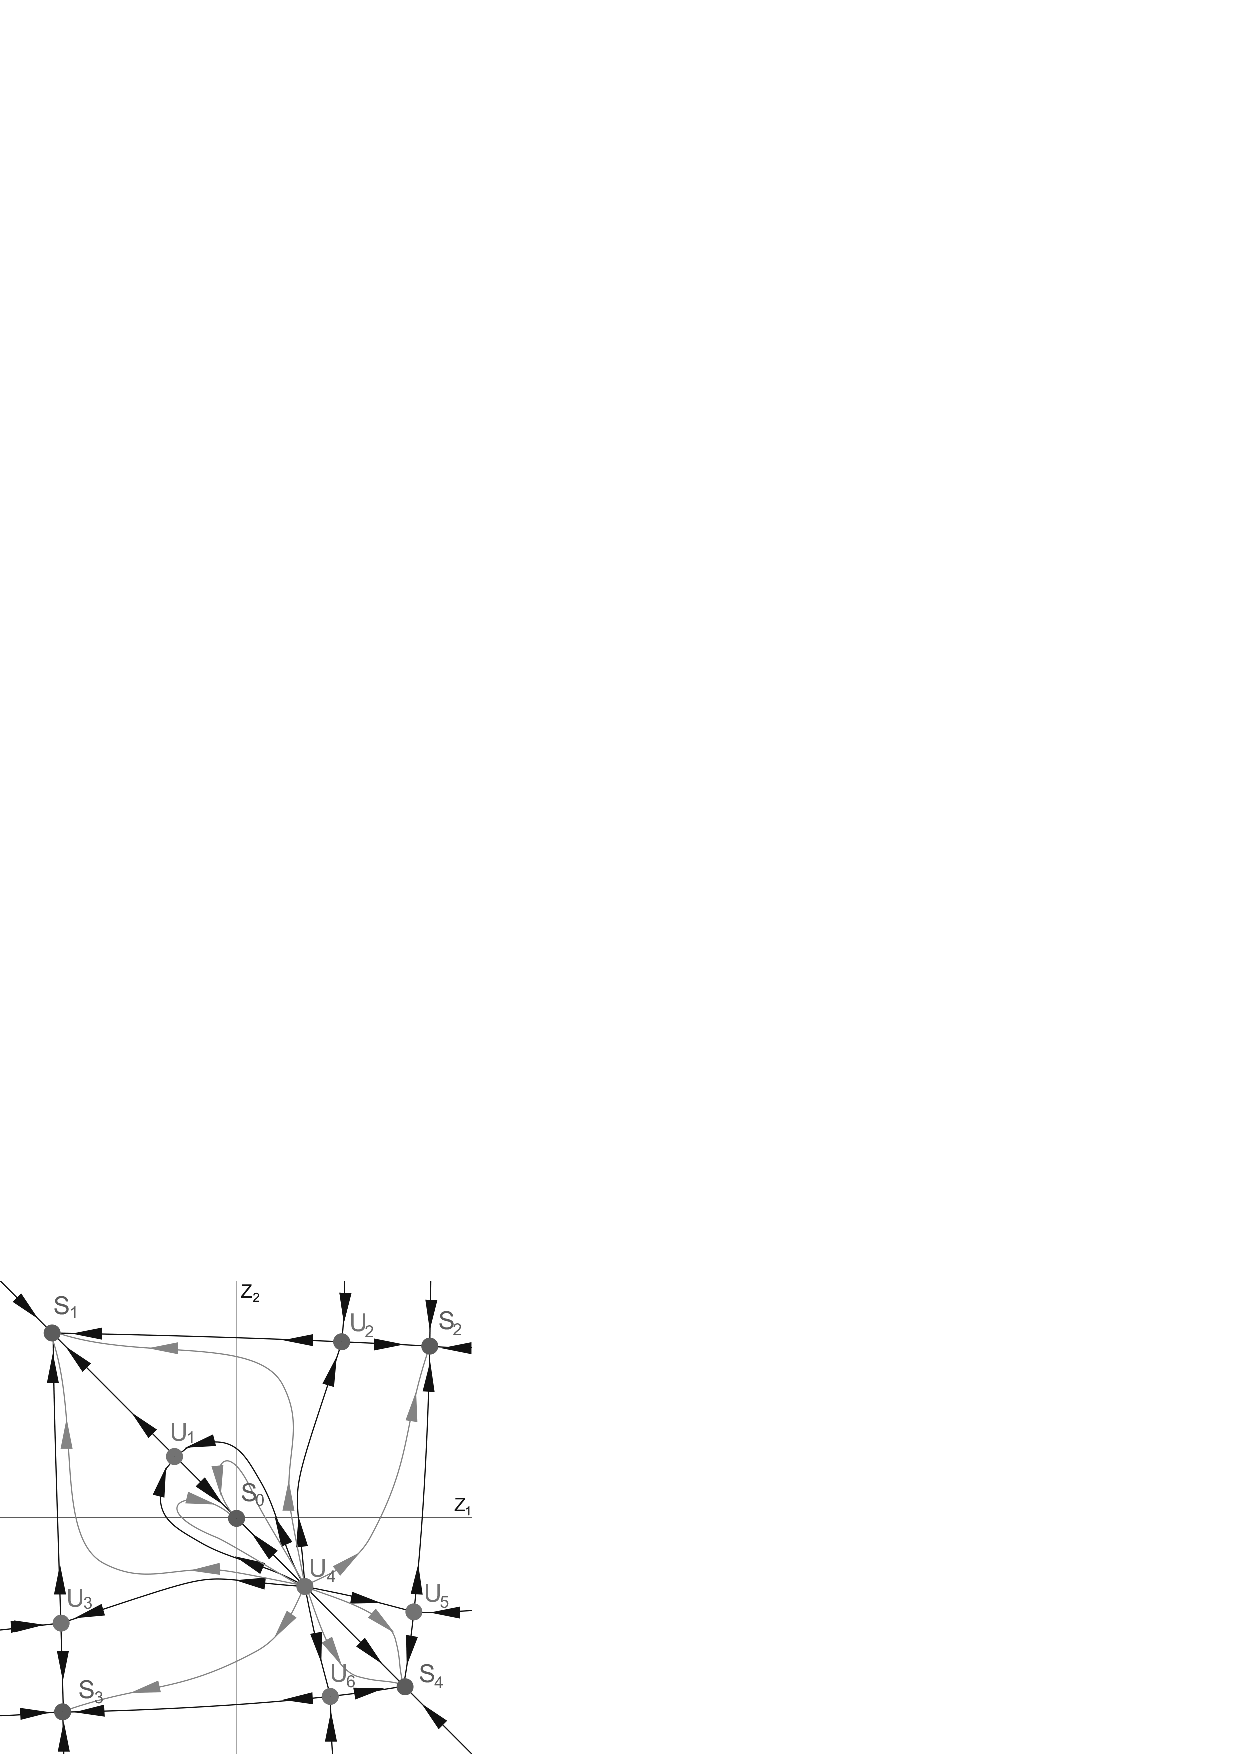
\includegraphics[width=0.76\linewidth]{neuman5.pdf} \\ a) $ \alpha = 5.0, \, \beta = 0.4, \, d = 0.01 $ }
	\end{minipage}
	\hspace{-4.5cm}
	\begin{minipage}[h]{0.37\linewidth}
	\center{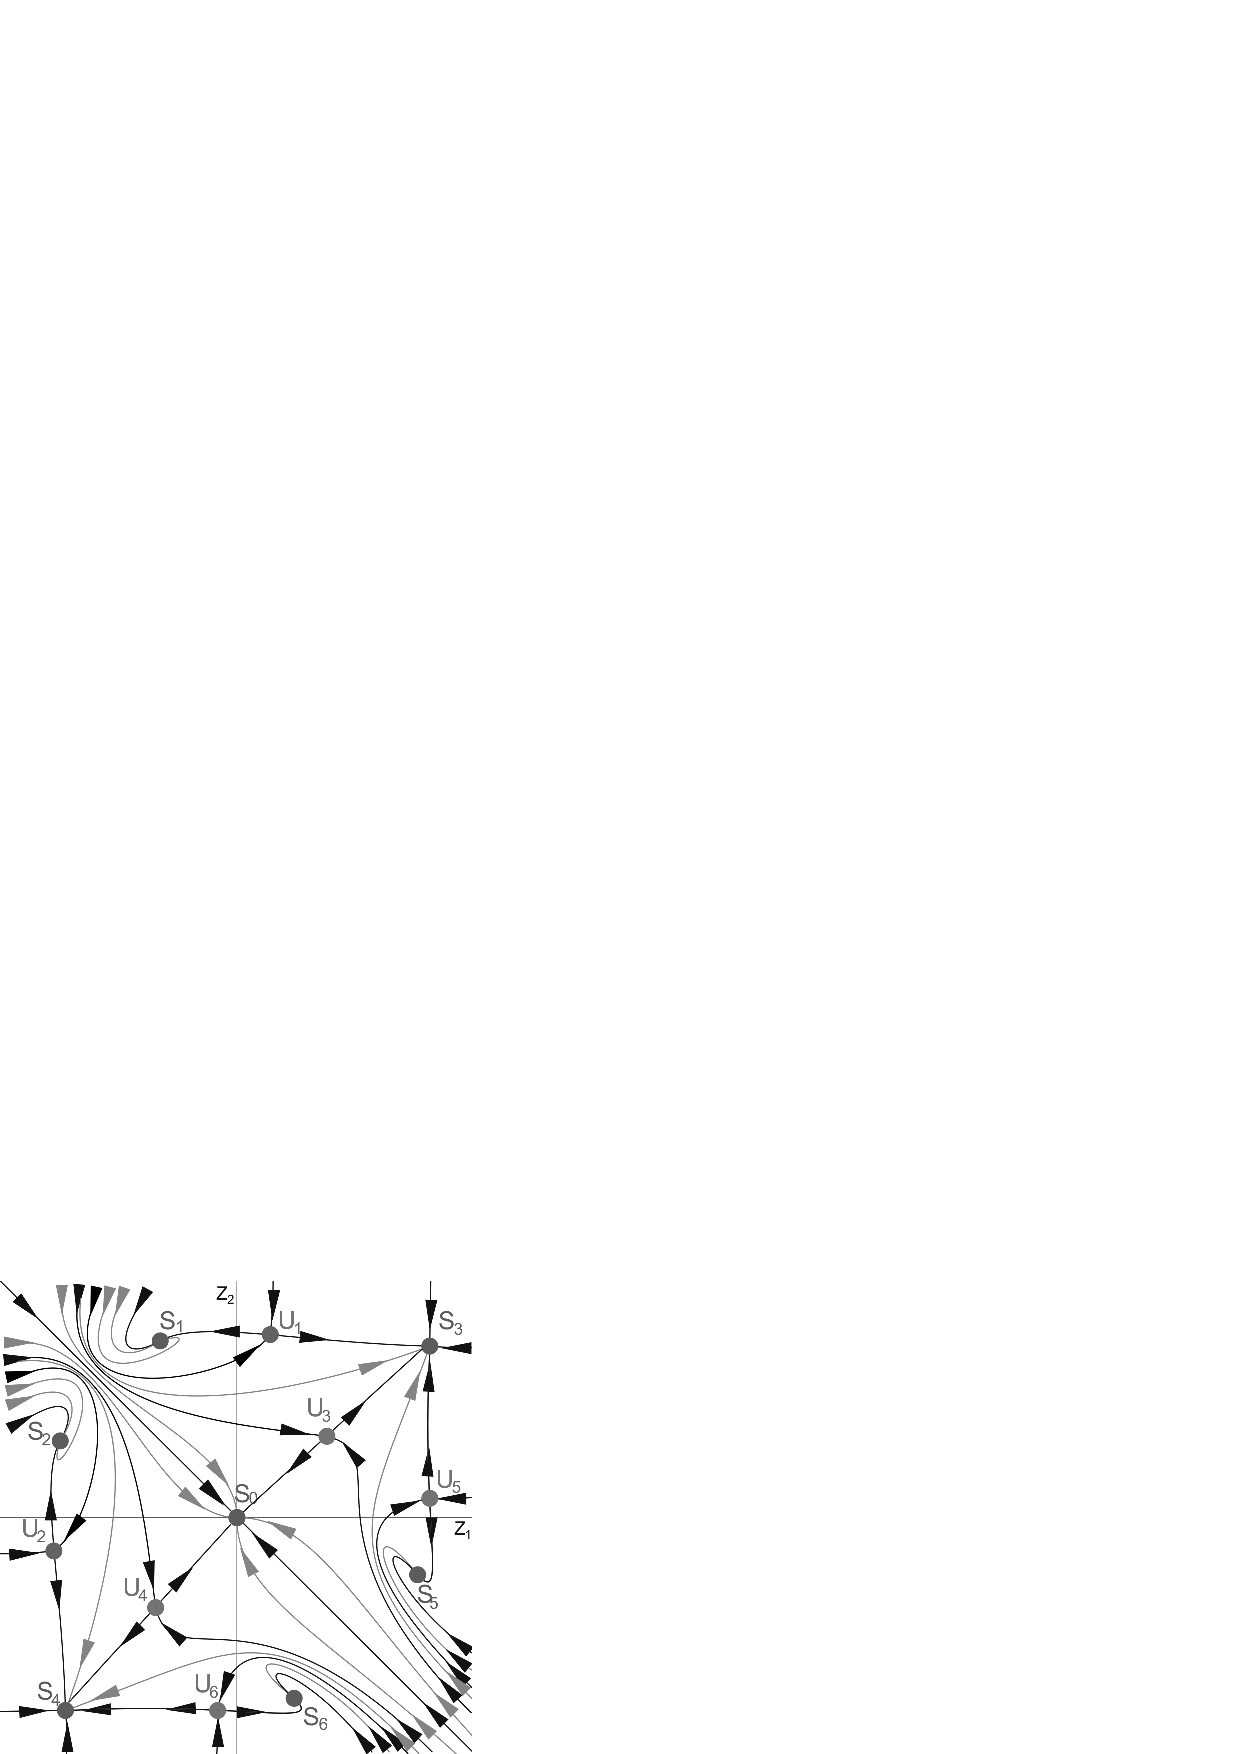
\includegraphics[width=0.76\linewidth]{neuman7.pdf} \\ b) $ \alpha = 5.0, \, \beta = 3.0, \, d = 0.056 $ }
	\end{minipage}
	\hspace{-4.5cm}
	\begin{minipage}[h]{0.37\linewidth}
	\center{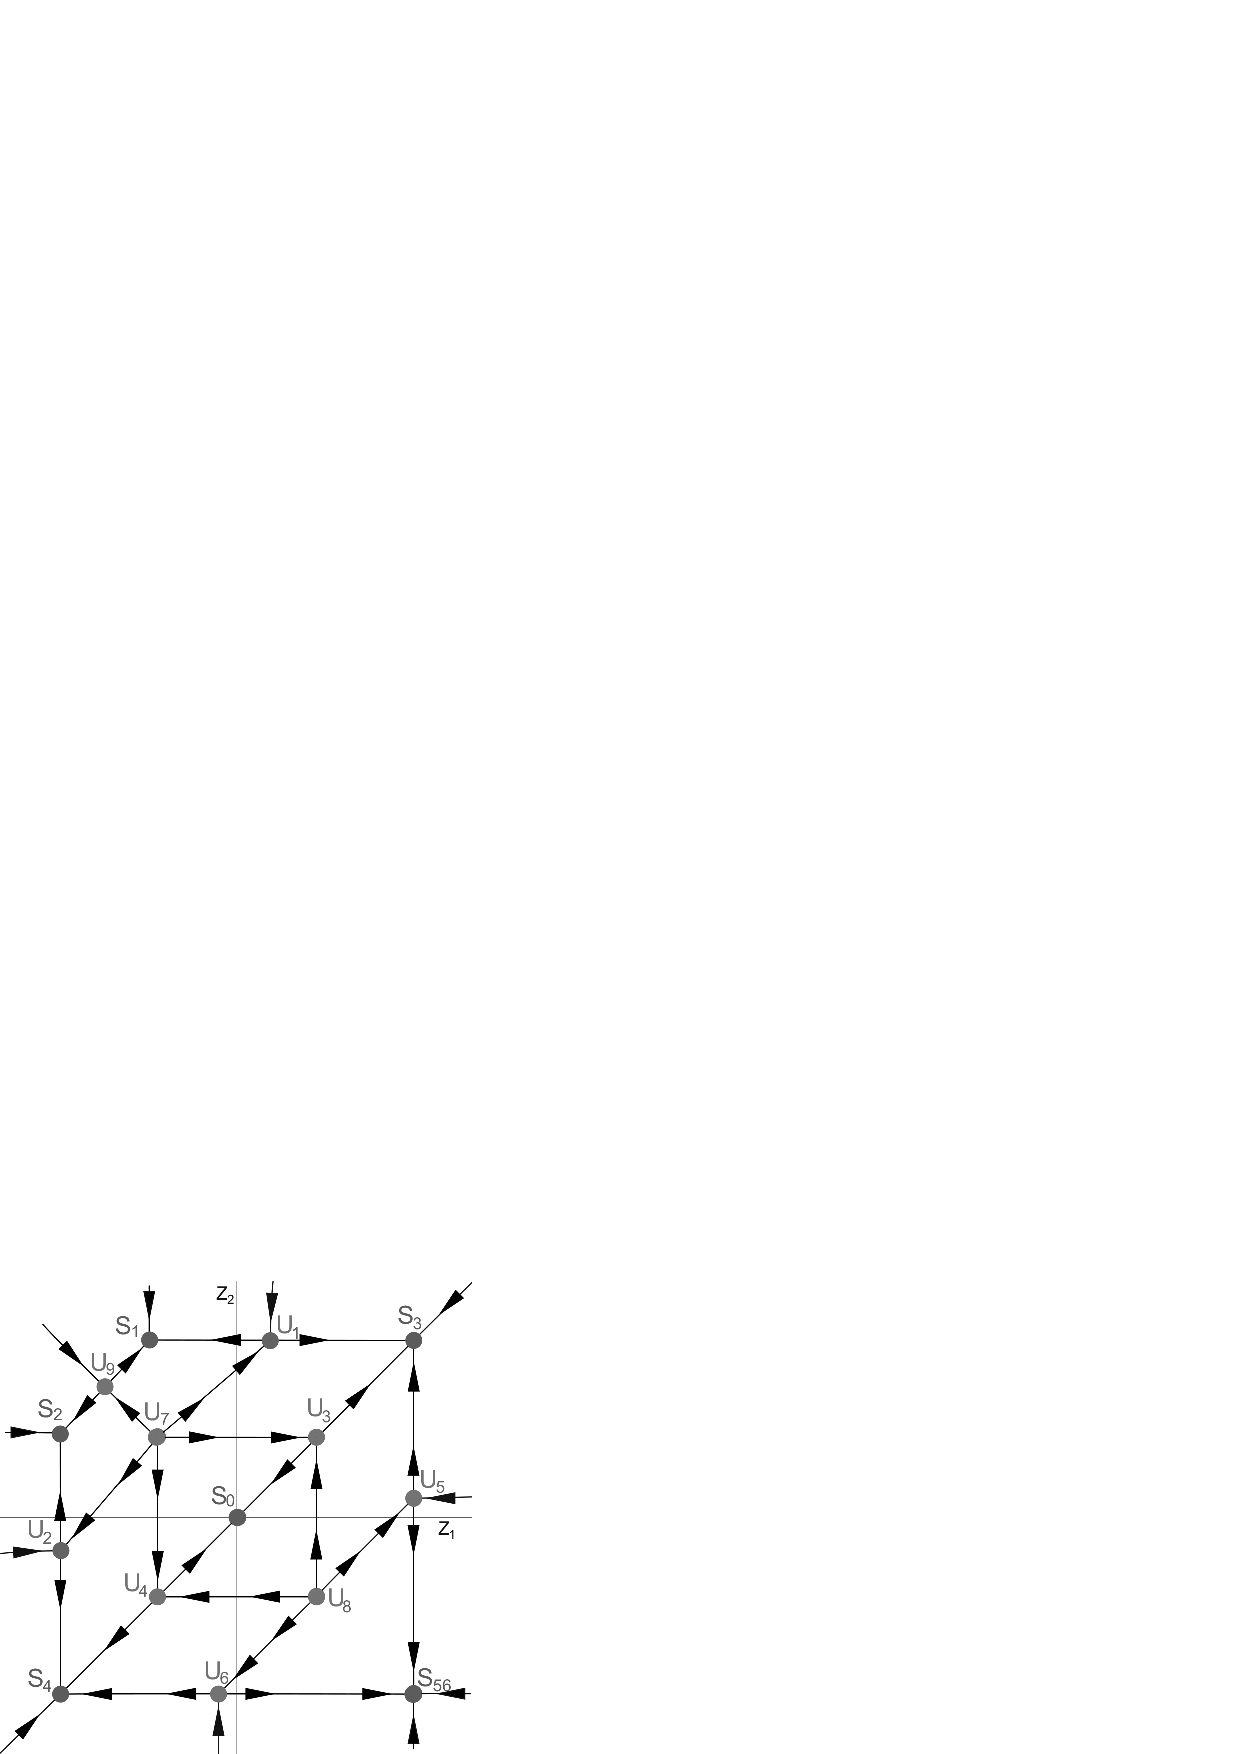
\includegraphics[width=0.76\linewidth]{neuman6.pdf} \\ c) $ \alpha = 4.0, \, \beta = 2.3, \, d = 0.045 $ }
	\end{minipage} 	
	
  } 

%%%%%%%%%% ------------------------------------------ %%%%%%%%%%
  \blocknodew{76}{Phase portraits in the case $ a_1 = 1, \, a_2 = 2; \, u_0 = u_3, \, u_1 = u_4 $ } %
  { 
	
\vspace{0.1cm}	
			
	\begin{minipage}[h]{0.37\linewidth}
	\center{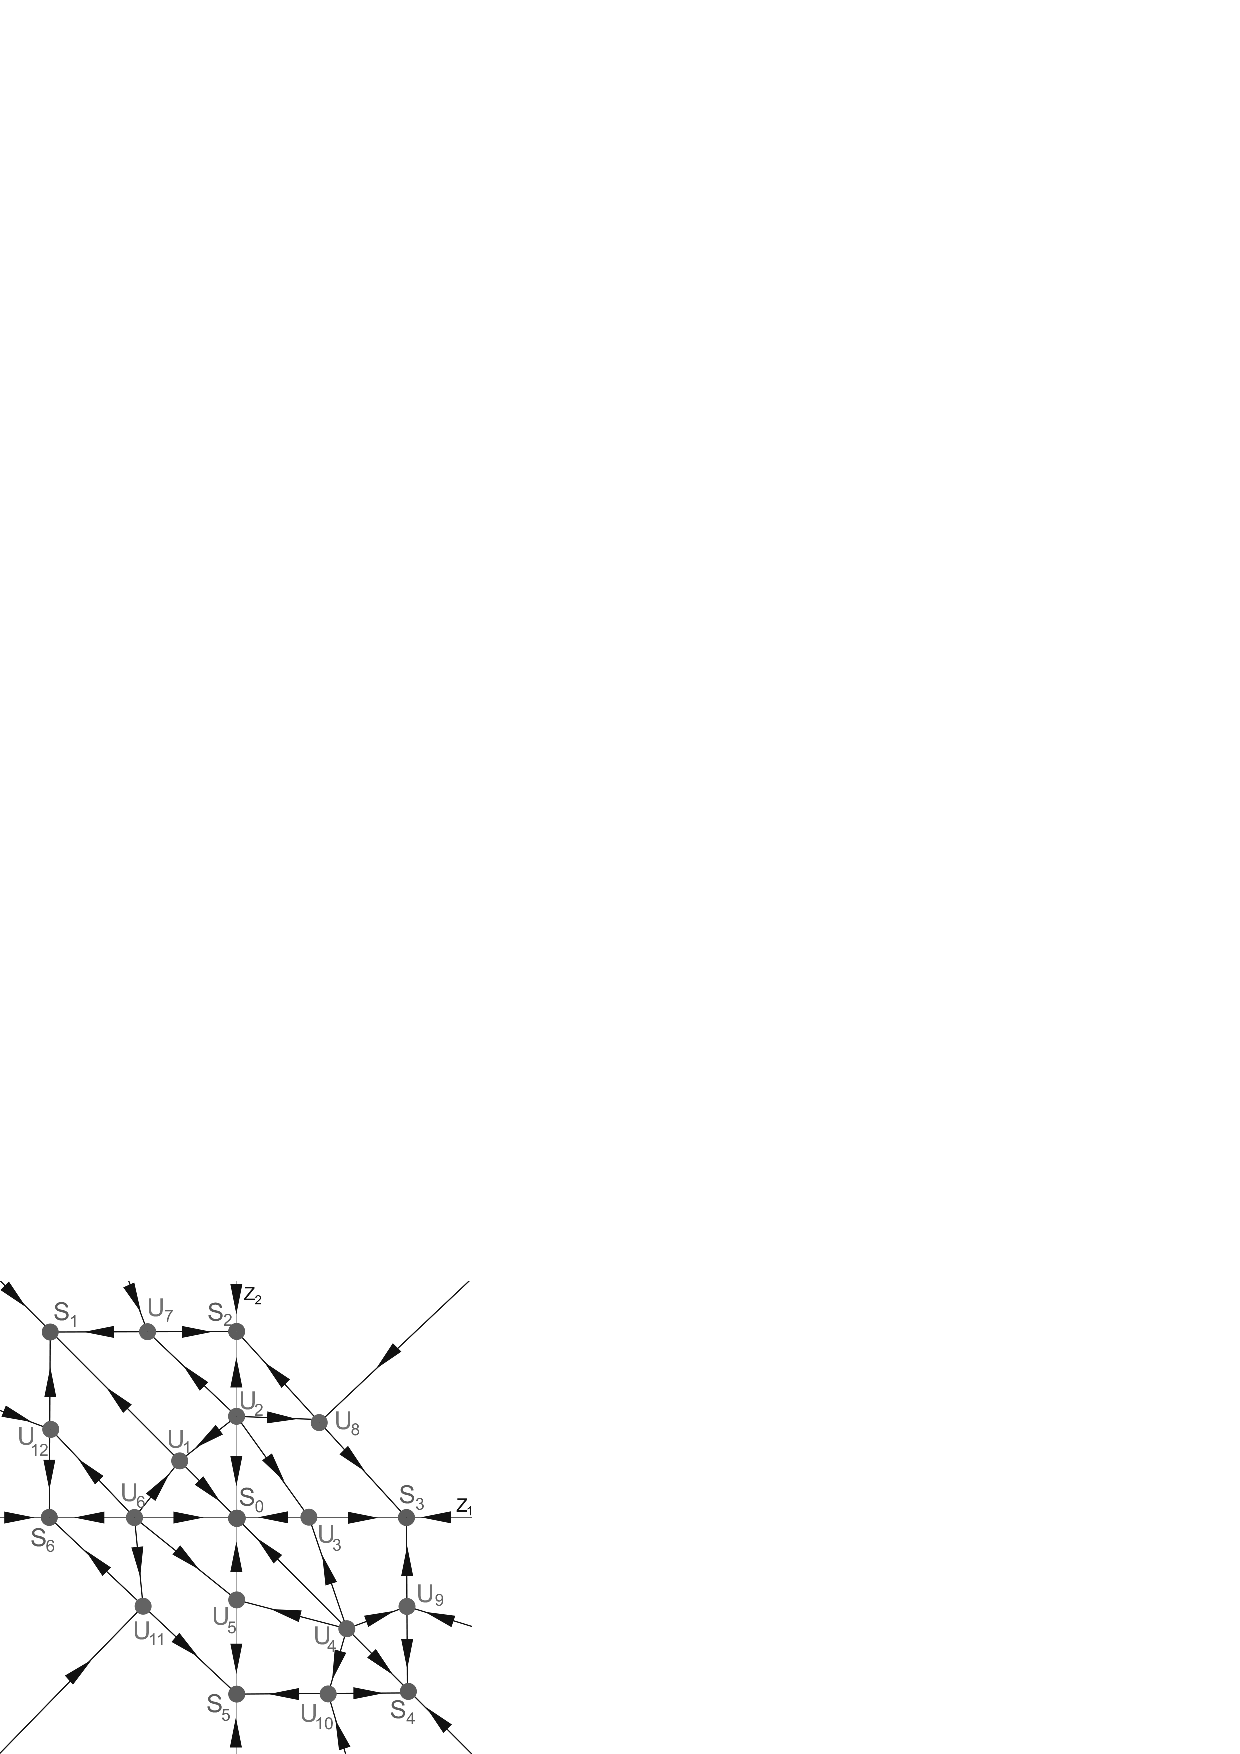
\includegraphics[width=0.76\linewidth]{periodic1.pdf} \\ a) $ \alpha = 5.0, \, \beta = 0.4, \, d = 0.005 $ }
	\end{minipage}
	\hspace{-4.5cm}
	\begin{minipage}[h]{0.37\linewidth}
	\center{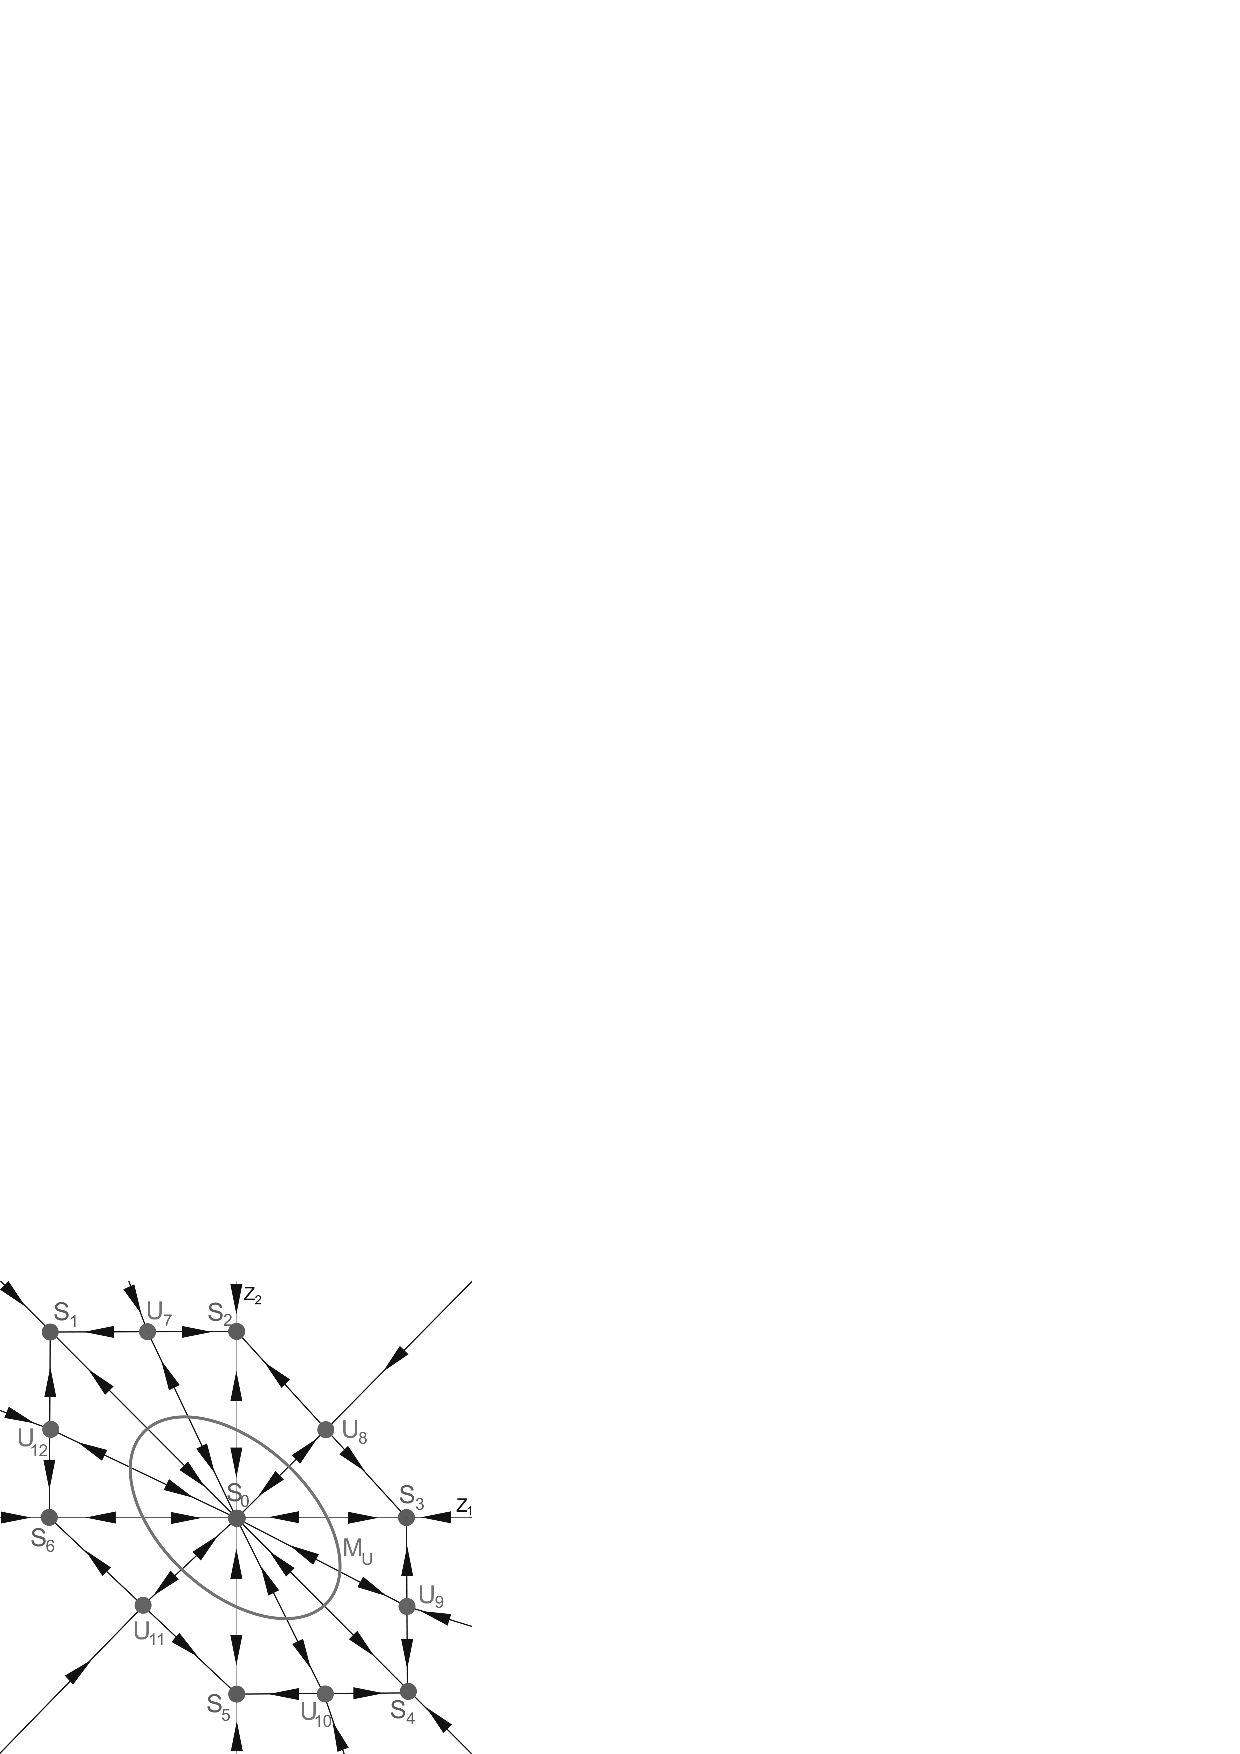
\includegraphics[width=0.76\linewidth]{periodictransarea.pdf} \\ b) $ \alpha = 5.0, \, \beta = 2.99, \, d = 0.04 $ }
	\end{minipage}
	\hspace{-4.5cm}
	\begin{minipage}[h]{0.37\linewidth}
	\center{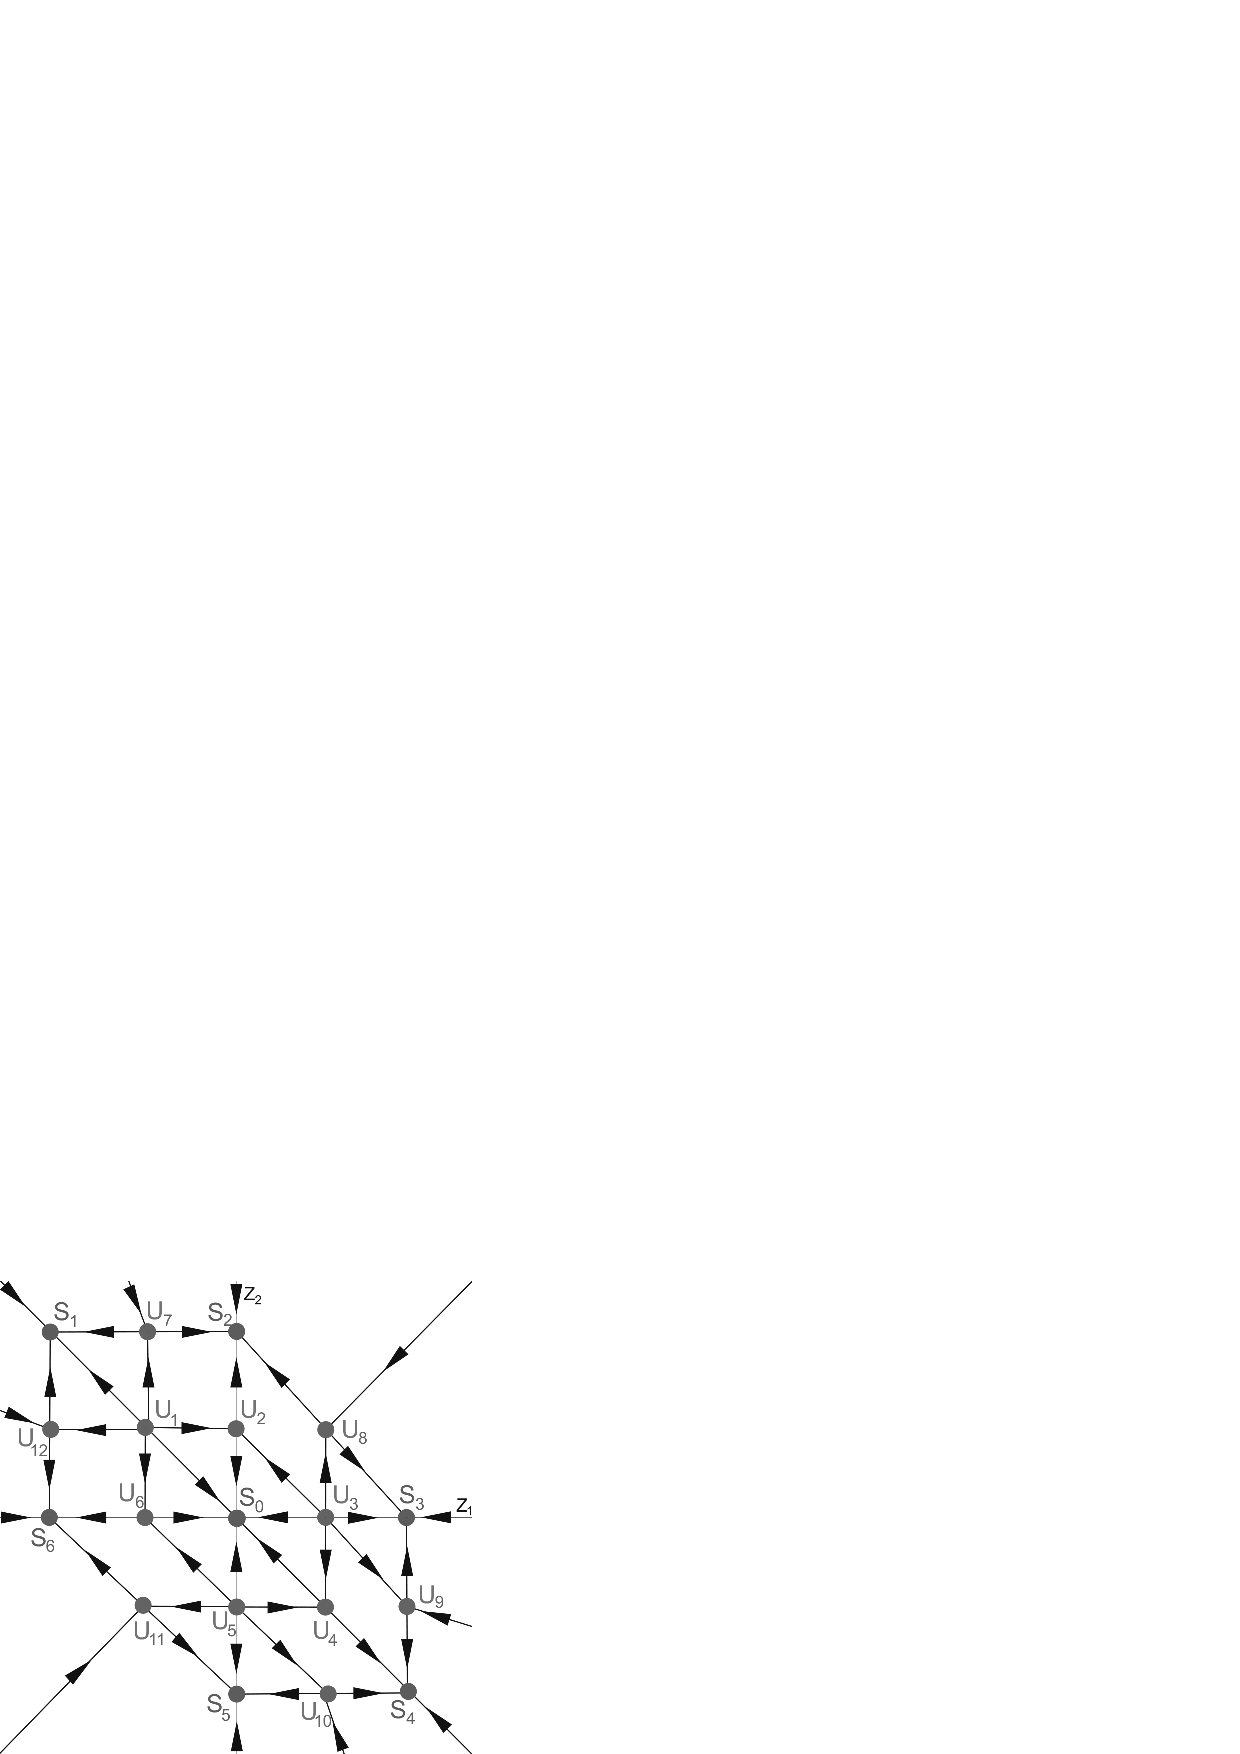
\includegraphics[width=0.76\linewidth]{periodic2.pdf} \\ c) $ \alpha = 4.0, \, \beta = 2.3, \, d = 0.03 $ }
	\end{minipage} 	
	
  } 

%%%%%%%%%% ------------------------------------------ %%%%%%%%%%
  \blocknodew{76}{Bifurcations in the case $ a_1 = 0, \, a_2 = 1; \, u_1 = u_4; \, \alpha = 1.9, \; \beta = 0.1 $ } %
  { 
	
\vspace{0.1cm}	
			
	\begin{minipage}[h]{0.34\linewidth}
	\center{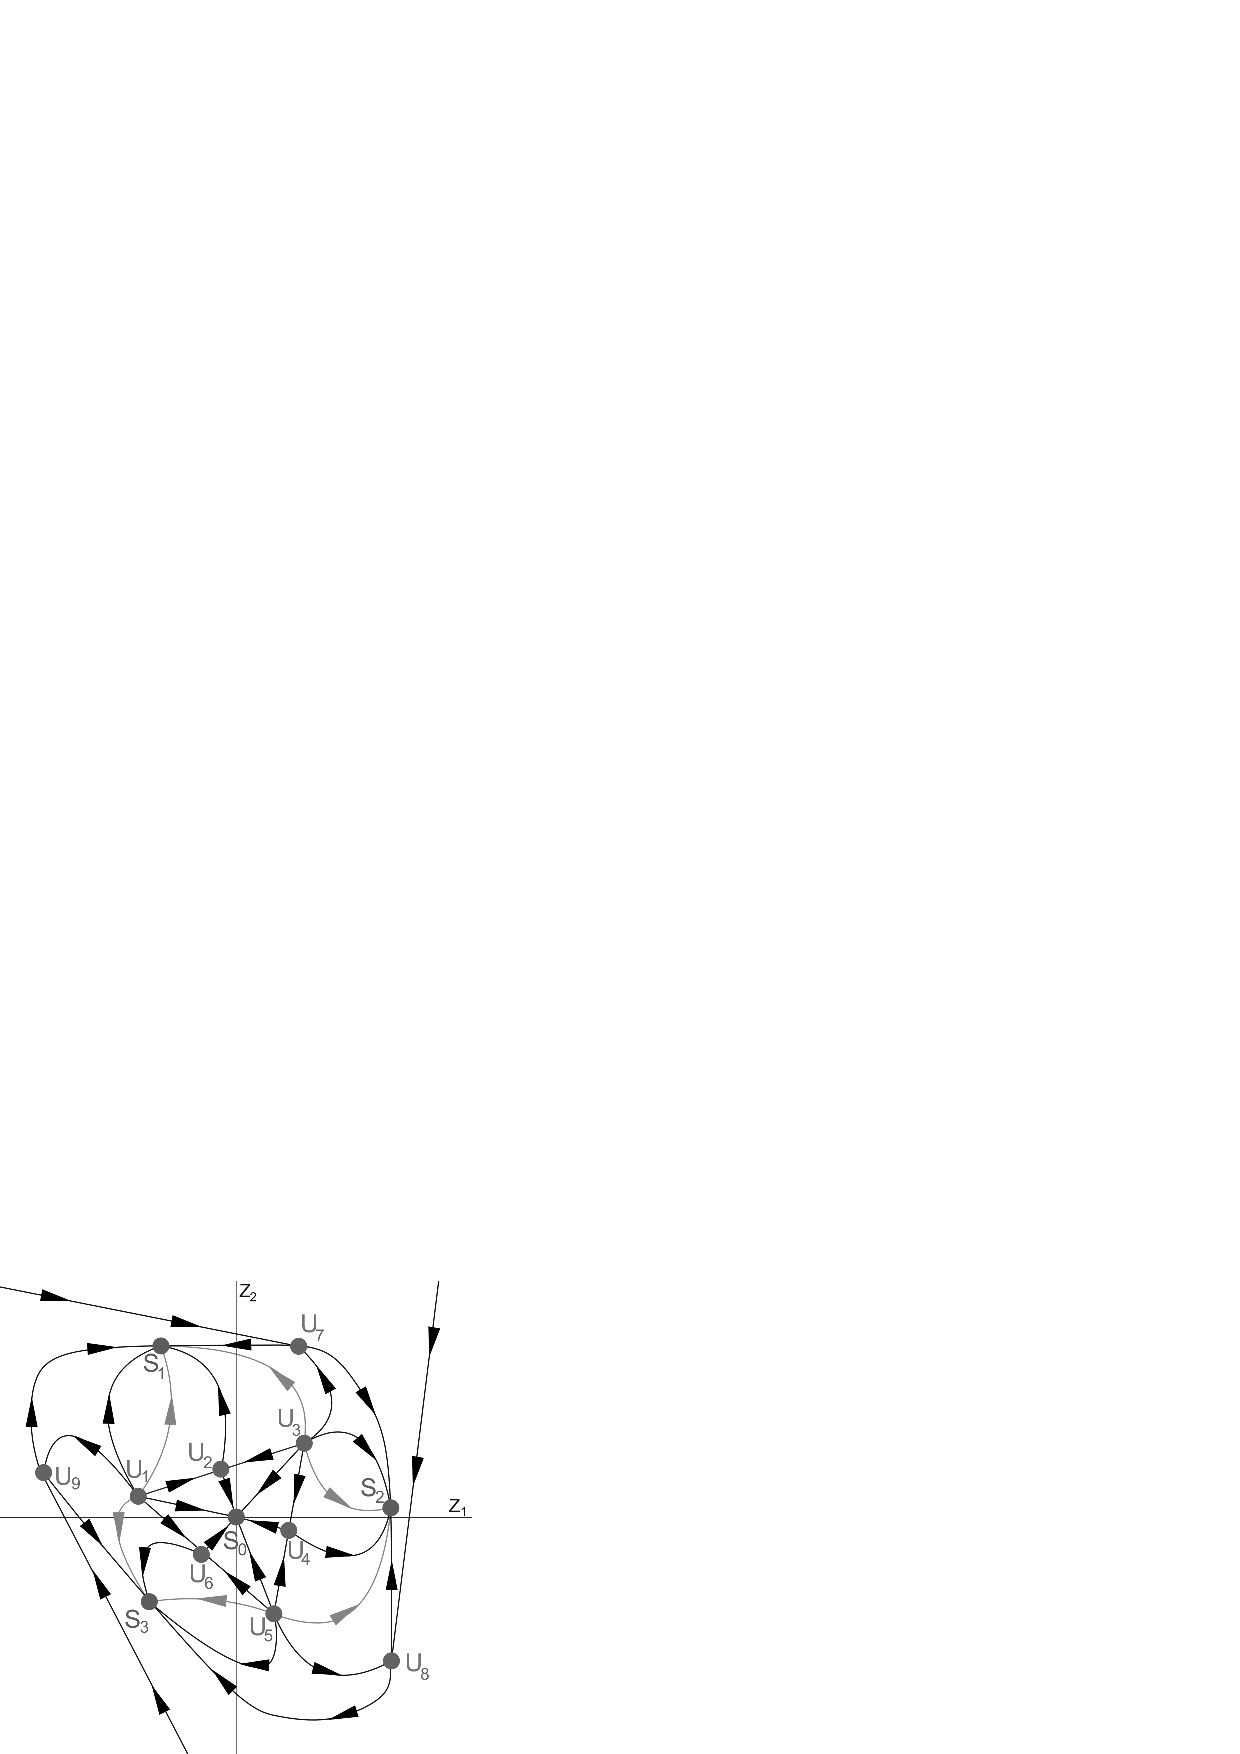
\includegraphics[width=0.64\linewidth]{uniwave1.pdf} \\ a) $ d < 0{,}316 $ }
	\end{minipage}
	\hspace{-9.0cm}
	\begin{minipage}[h]{0.34\linewidth}
	\center{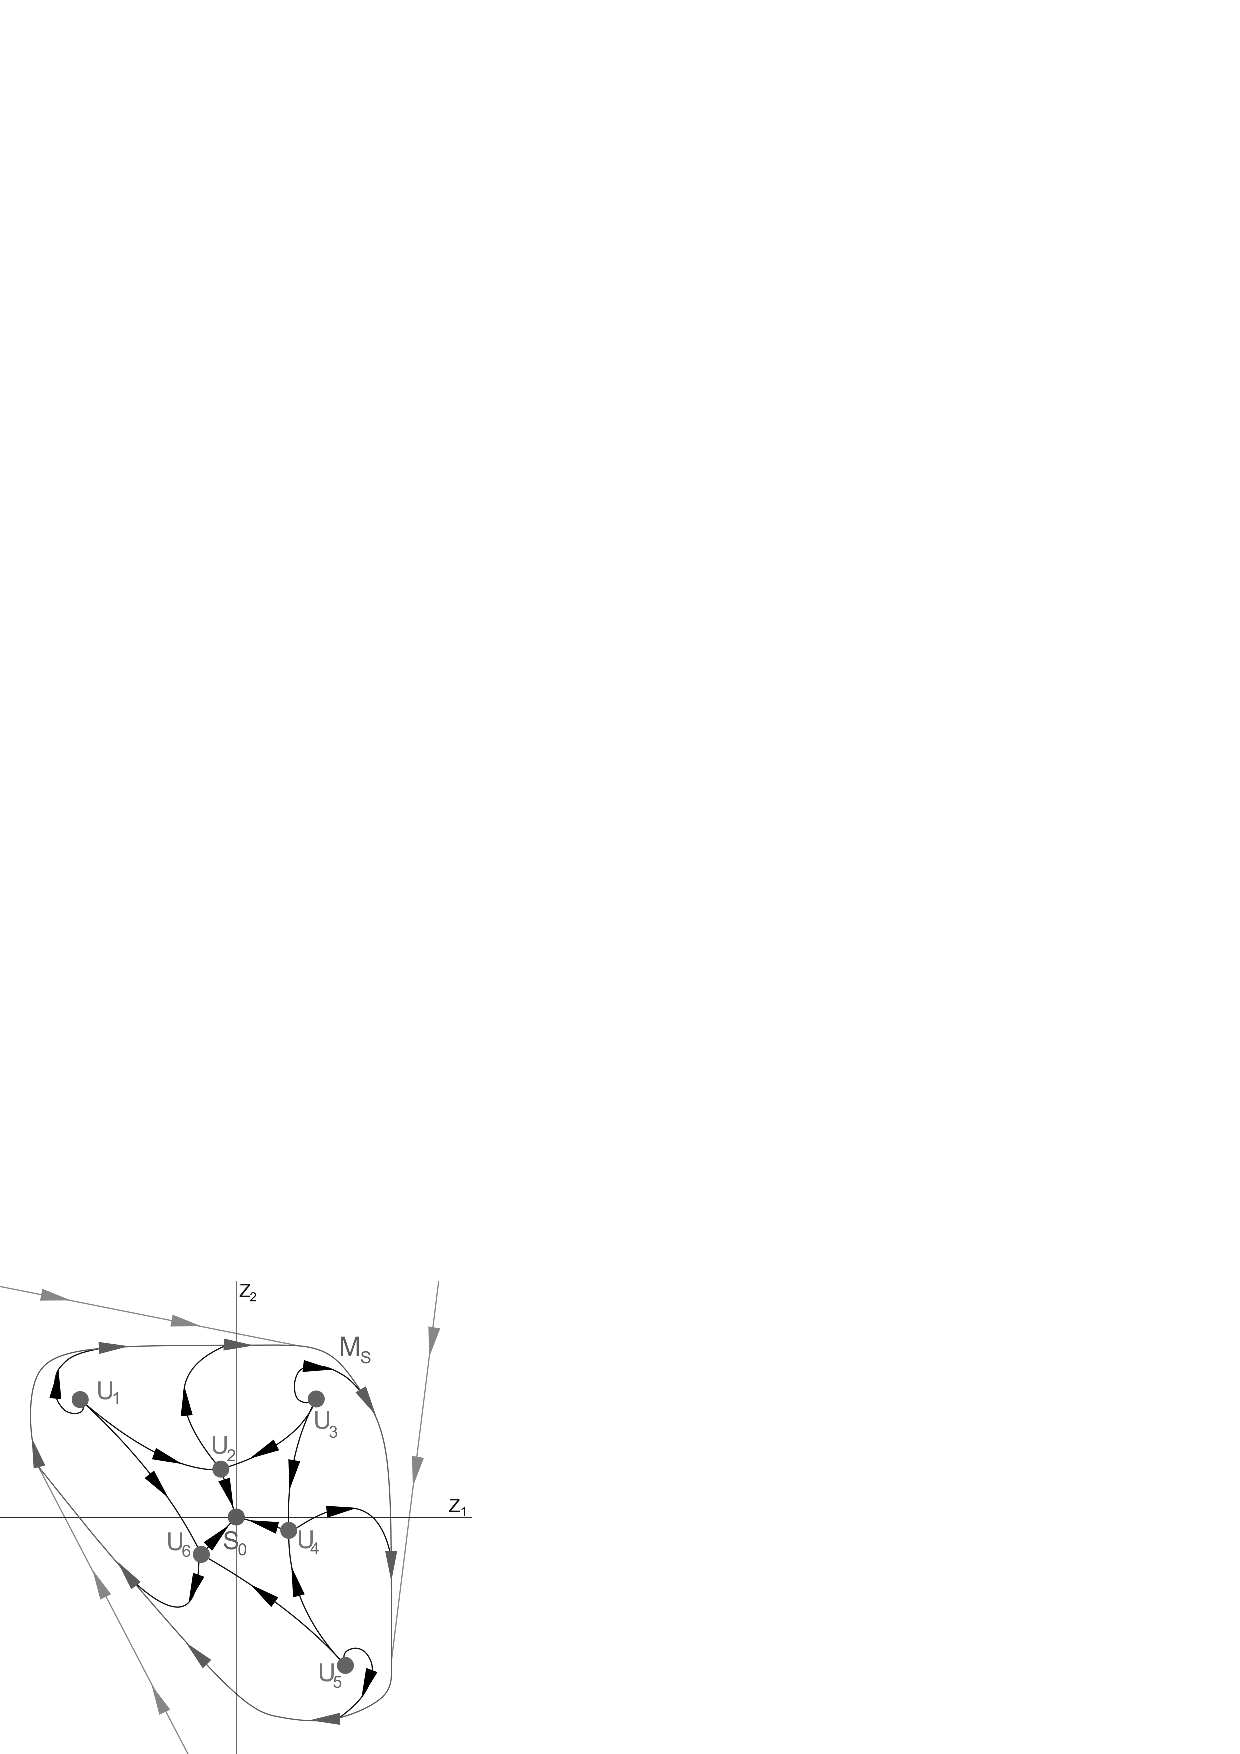
\includegraphics[width=0.64\linewidth]{uniwave2.pdf} \\ b) $ 0{,}316 \leqslant d < 0{,}317 $ }
	\end{minipage}
	\hspace{-9.0cm}
	\begin{minipage}[h]{0.34\linewidth}
	\center{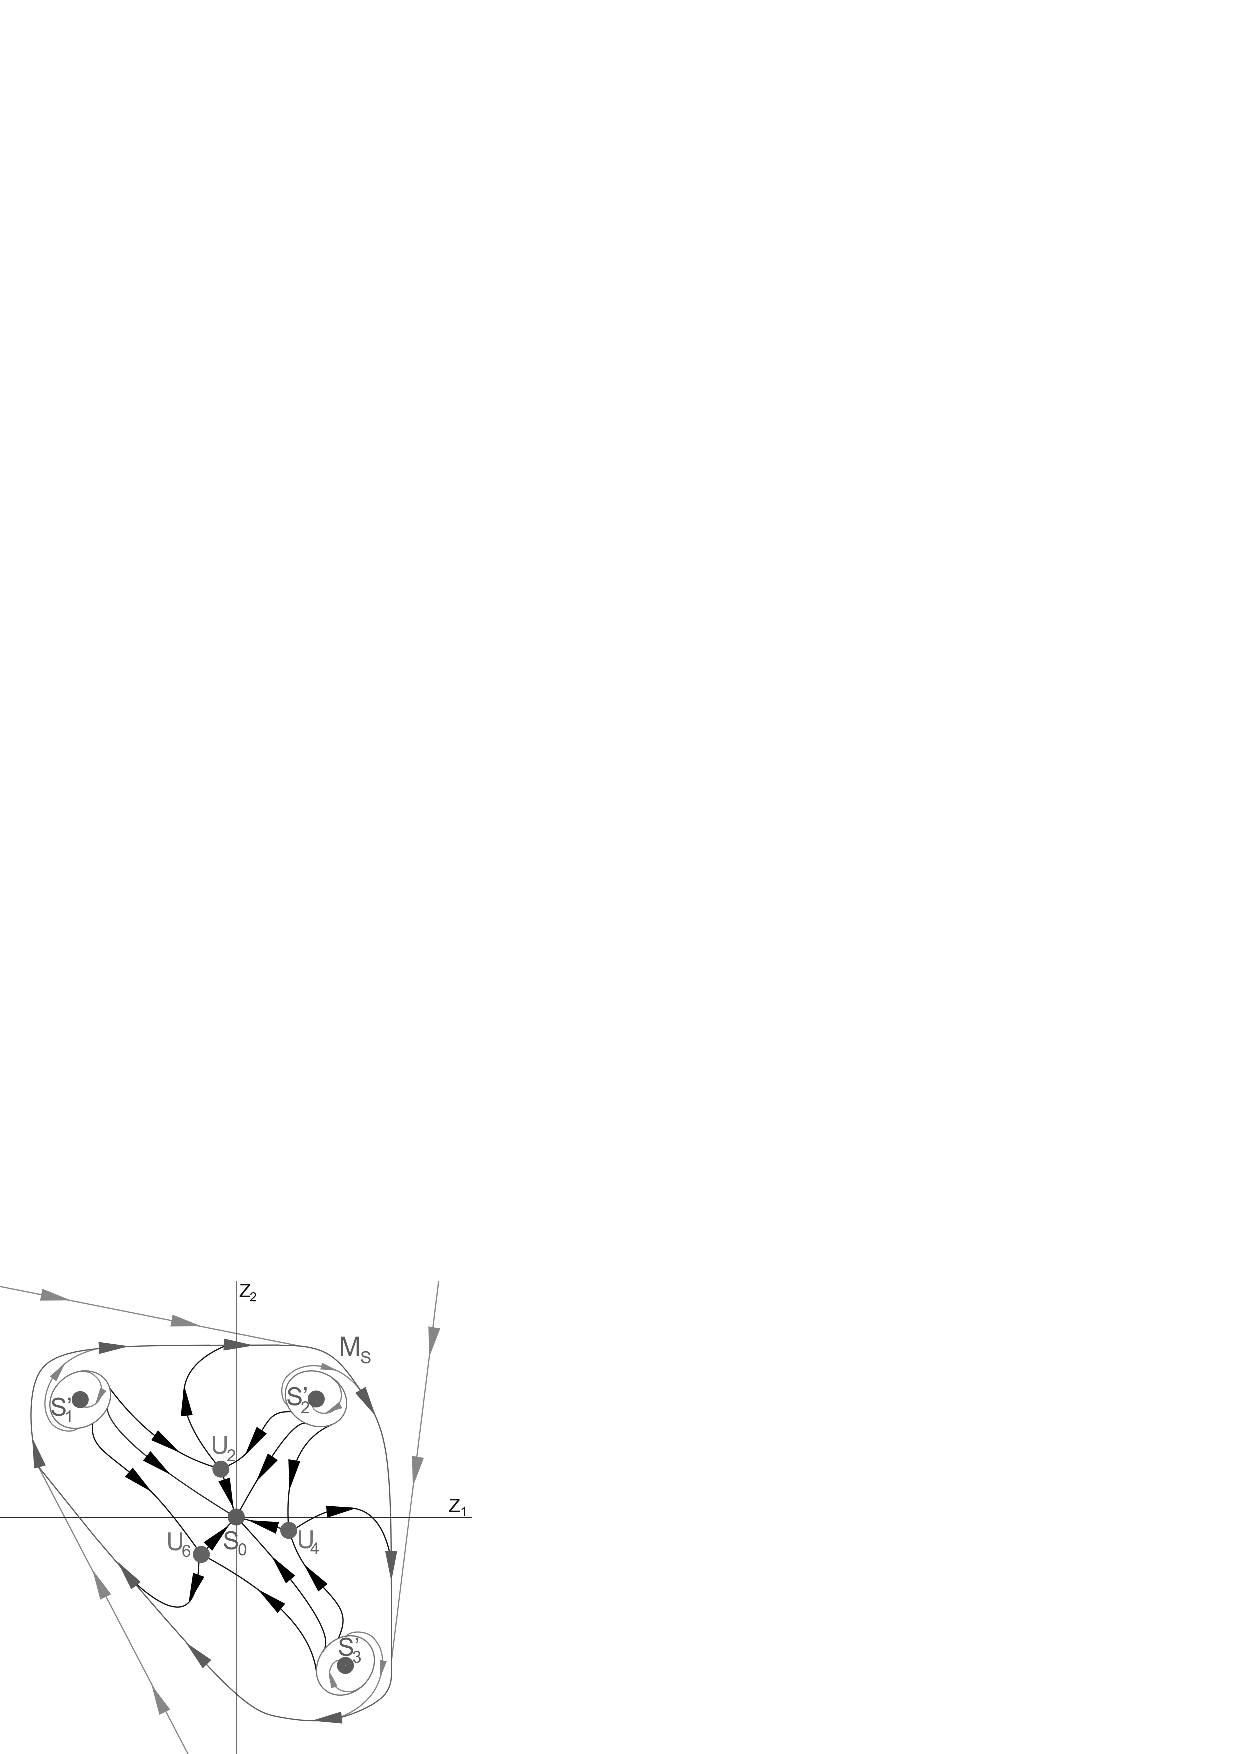
\includegraphics[width=0.64\linewidth]{uniwave3.pdf} \\ c) $ 0{,}317 \leqslant d < 0{,}3174 $ }
	\end{minipage} 
	\hspace{-9.0cm}
	\begin{minipage}[h]{0.34\linewidth}
	\center{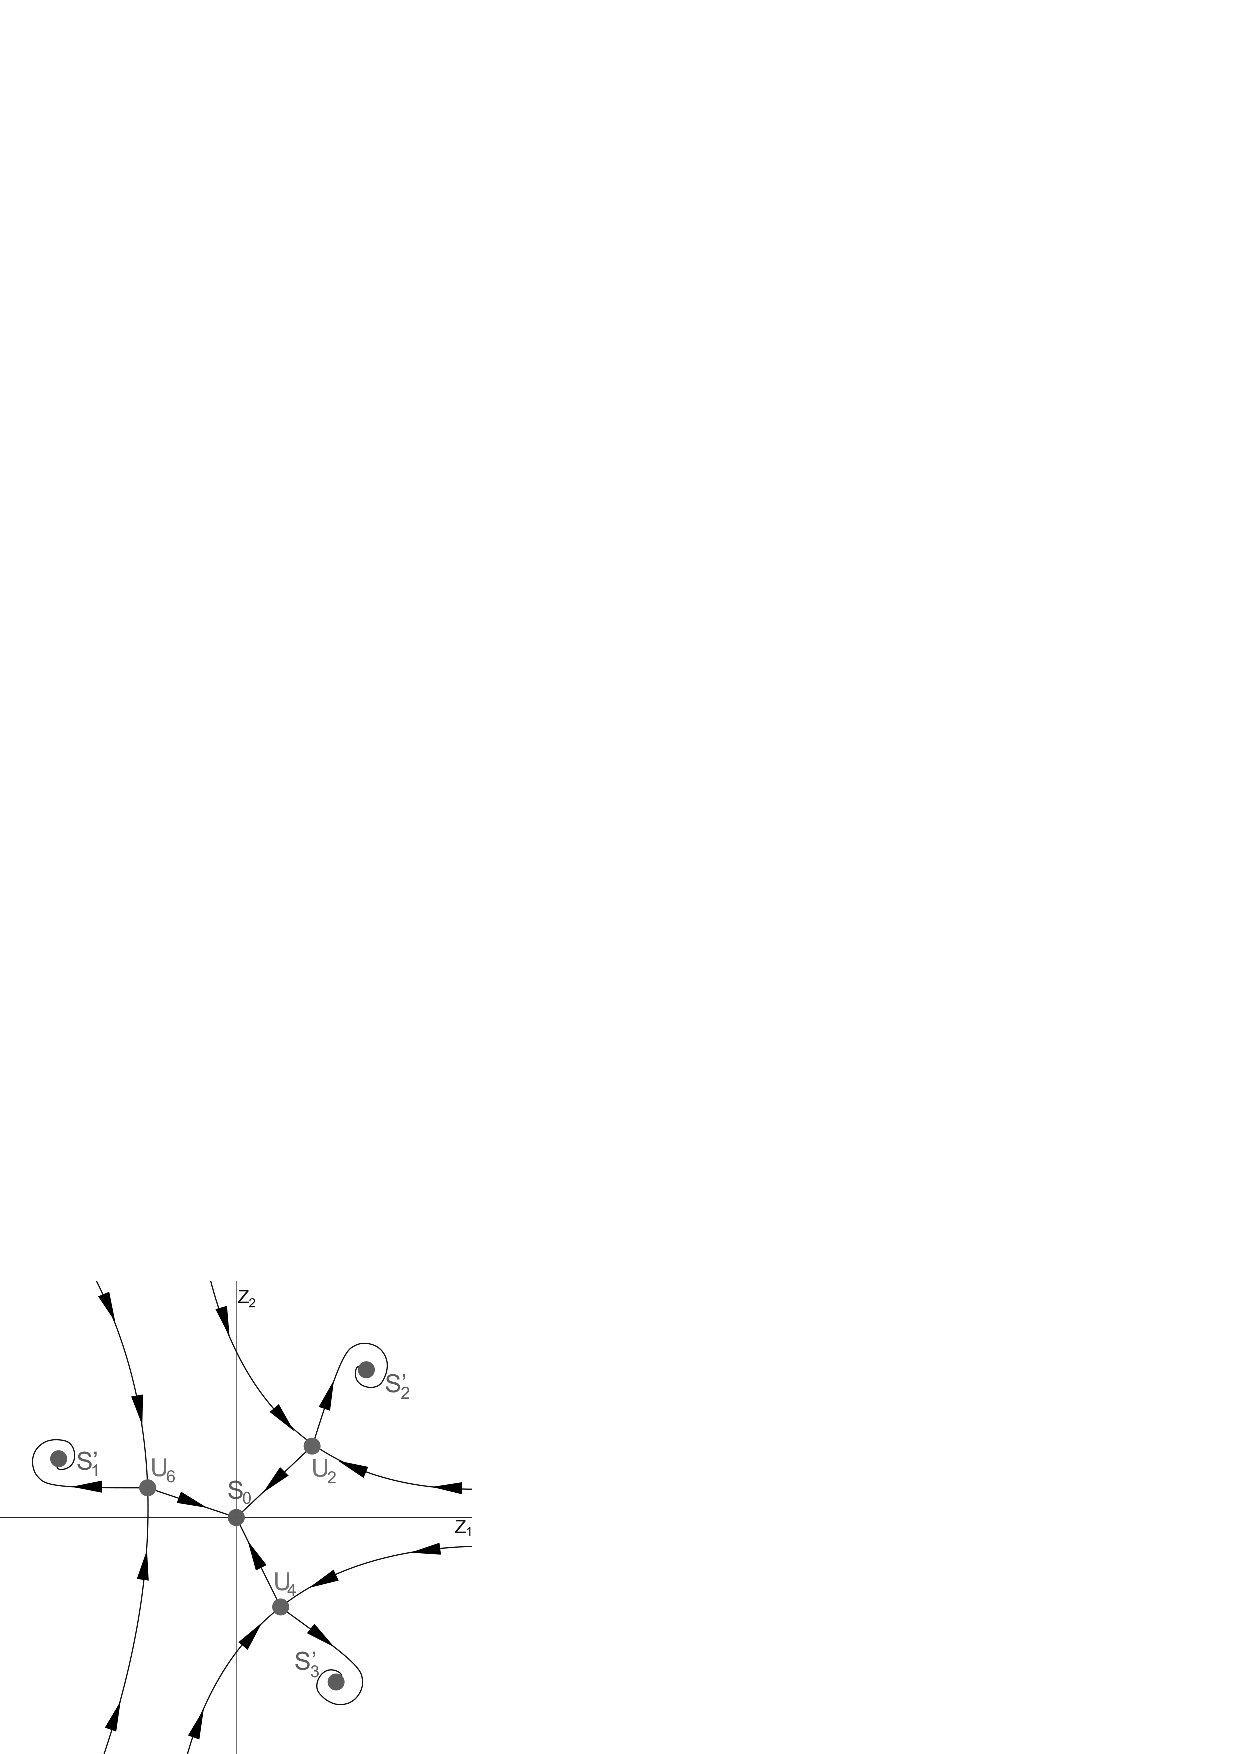
\includegraphics[width=0.64\linewidth]{uniwave4.pdf} \\ d) $ 0{,}3174 \leqslant d < 0{,}3178 $ }
	\end{minipage}	
	
  } 

  %%%%%%%%%%%%% NEW COLUMN %%%%%%%%%%%%%%% 
  \startsecondcolumn 

%%%%%%%%%% ------------------------------------------ %%%%%%%%%%
  \blocknodew{37}{Research map} %
  {
	\begin{equation}
	\Phi(z): \begin{pmatrix}
           z_1 \\
           z_2
          \end{pmatrix}
					\to
					\begin{pmatrix}
           y_1(T_0) \\
           y_2(T_0)
          \end{pmatrix},
	\end{equation}
	
	$$ y_1(-0) = z_1, \; y_2(-0) = z_2, $$
	$$ y_j \approx \mbox{ln}\, u_{j+1} - \mbox{ln}\, u_j, \quad j = \overline{1,2} $$
	$$ T_0 = \alpha + 1 + (\beta+1)/(\alpha - \beta - 1). $$

	\vspace{0.7cm}

  }

\end{tikzpicture}

\end{document}